\chapter{Configurations et transformations élémentaires du plan}
%\stepcounter{module}

{\AlegreyaSansLight \large
\begin{center}
\textbf{Crédit :} 46 heures\\
\textit{4 heures hebdomadaires}
\end{center}
}

\minitoc

\section{Introduction}

\subsection{Présentation du module}
Ce module comporte deux parties essentielles : les configurations planes, les symétries orthogonales et centrales dans le plan. Il développe deux compétences fondamentales que sont :
\begin{itemize}
\item déployer un raisonnement mathématique (analogique, inductif et déductif);
\item résoudre des problèmes par l'observation, l'identification et la caractérisation des formes planes ; par les transformations élémentaires que sont les symétries.
\end{itemize}
Il s'articule sur la famille de situations suivante : représentations et transformations des configurations planes dans l'environnement. Les compétences mises en contexte s'appuient sur les trois catégories d'actions que sont :
\begin{itemize}
\item Perception des formes planes et des transformations dans l'environnement physique.
\item Production des formes planes et des transformations dans l'environnement physique.
\item Détermination des mesures et des positions dans l'environnement.\\
Cette dernière catégorie d'actions est le champ privilégié de l'inter action entre les activités numériques et les activités géométriques de l’élève de 5ème .\\
Les différentes actions qui s'intègrent dans chacune des catégories suscitées sont en corrélation avec les savoirs essentiels que ce module développe, et qui s'appuient sur les habiletés cognitives suivantes : connaissance, compréhension et application.
\end{itemize}

\subsection{Contribution du module à la finalité et aux buts curriculaires}
A travers les différents raisonnements sus évoqués, l'apprenant développe les compétences transversales suivantes : le sens de l'ordre, le sens de la rigueur et de la concision (en intégrant, dans le cadre d'une démarche scientifique, chacune des méthodes utilisées pour le traitement compétent des situations de vie), la pensée
critique, le sens de l'initiative et de la créativité. Autant d'attitudes qui contribuent à la formation d'un citoyen autonome et responsable dans l'exercice de ses rôles sociaux.

\subsection{Contribution du module au programme d'études et aux domaines de vie}
La géométrie plane occupe une place privilégiée dans le programme de mathématiques de par les compétences qu'elle vise à développer. Sa contribution au développement de la technologie, de l'art, de la chimie, ne sont plus à démontrer ; enfin les innombrables symétries que la nature offre dans la biologie et la physiologie végétale ou animale font de ce module un des maillons essentiels dans plus d'un domaine d'apprentissage.\\
L'importance de ce module réside dans le fait que l'élève vit dans un espace géographique. L'utilisation et la rencontre des objets dans lesquels on peut extraire des formes géométriques planes font partie du quotidien : aménagement ou réalisation de son habitat, manipulation ou réalisation de certains objets usuels, appréciation ou production des œuvres d'art, choix du chemin adéquat pour se rendre à un lieu pour ne citer que ceux-ci ; toutes choses pouvant l'aider à s'affirmer comme membre responsable d'une famille, à opérer des choix judicieux dans la consommation des biens , des services et de l'information. La contribution de ce module à tous les domaines de vie est donc d'une évidence incontestable.

\section{Matrice}

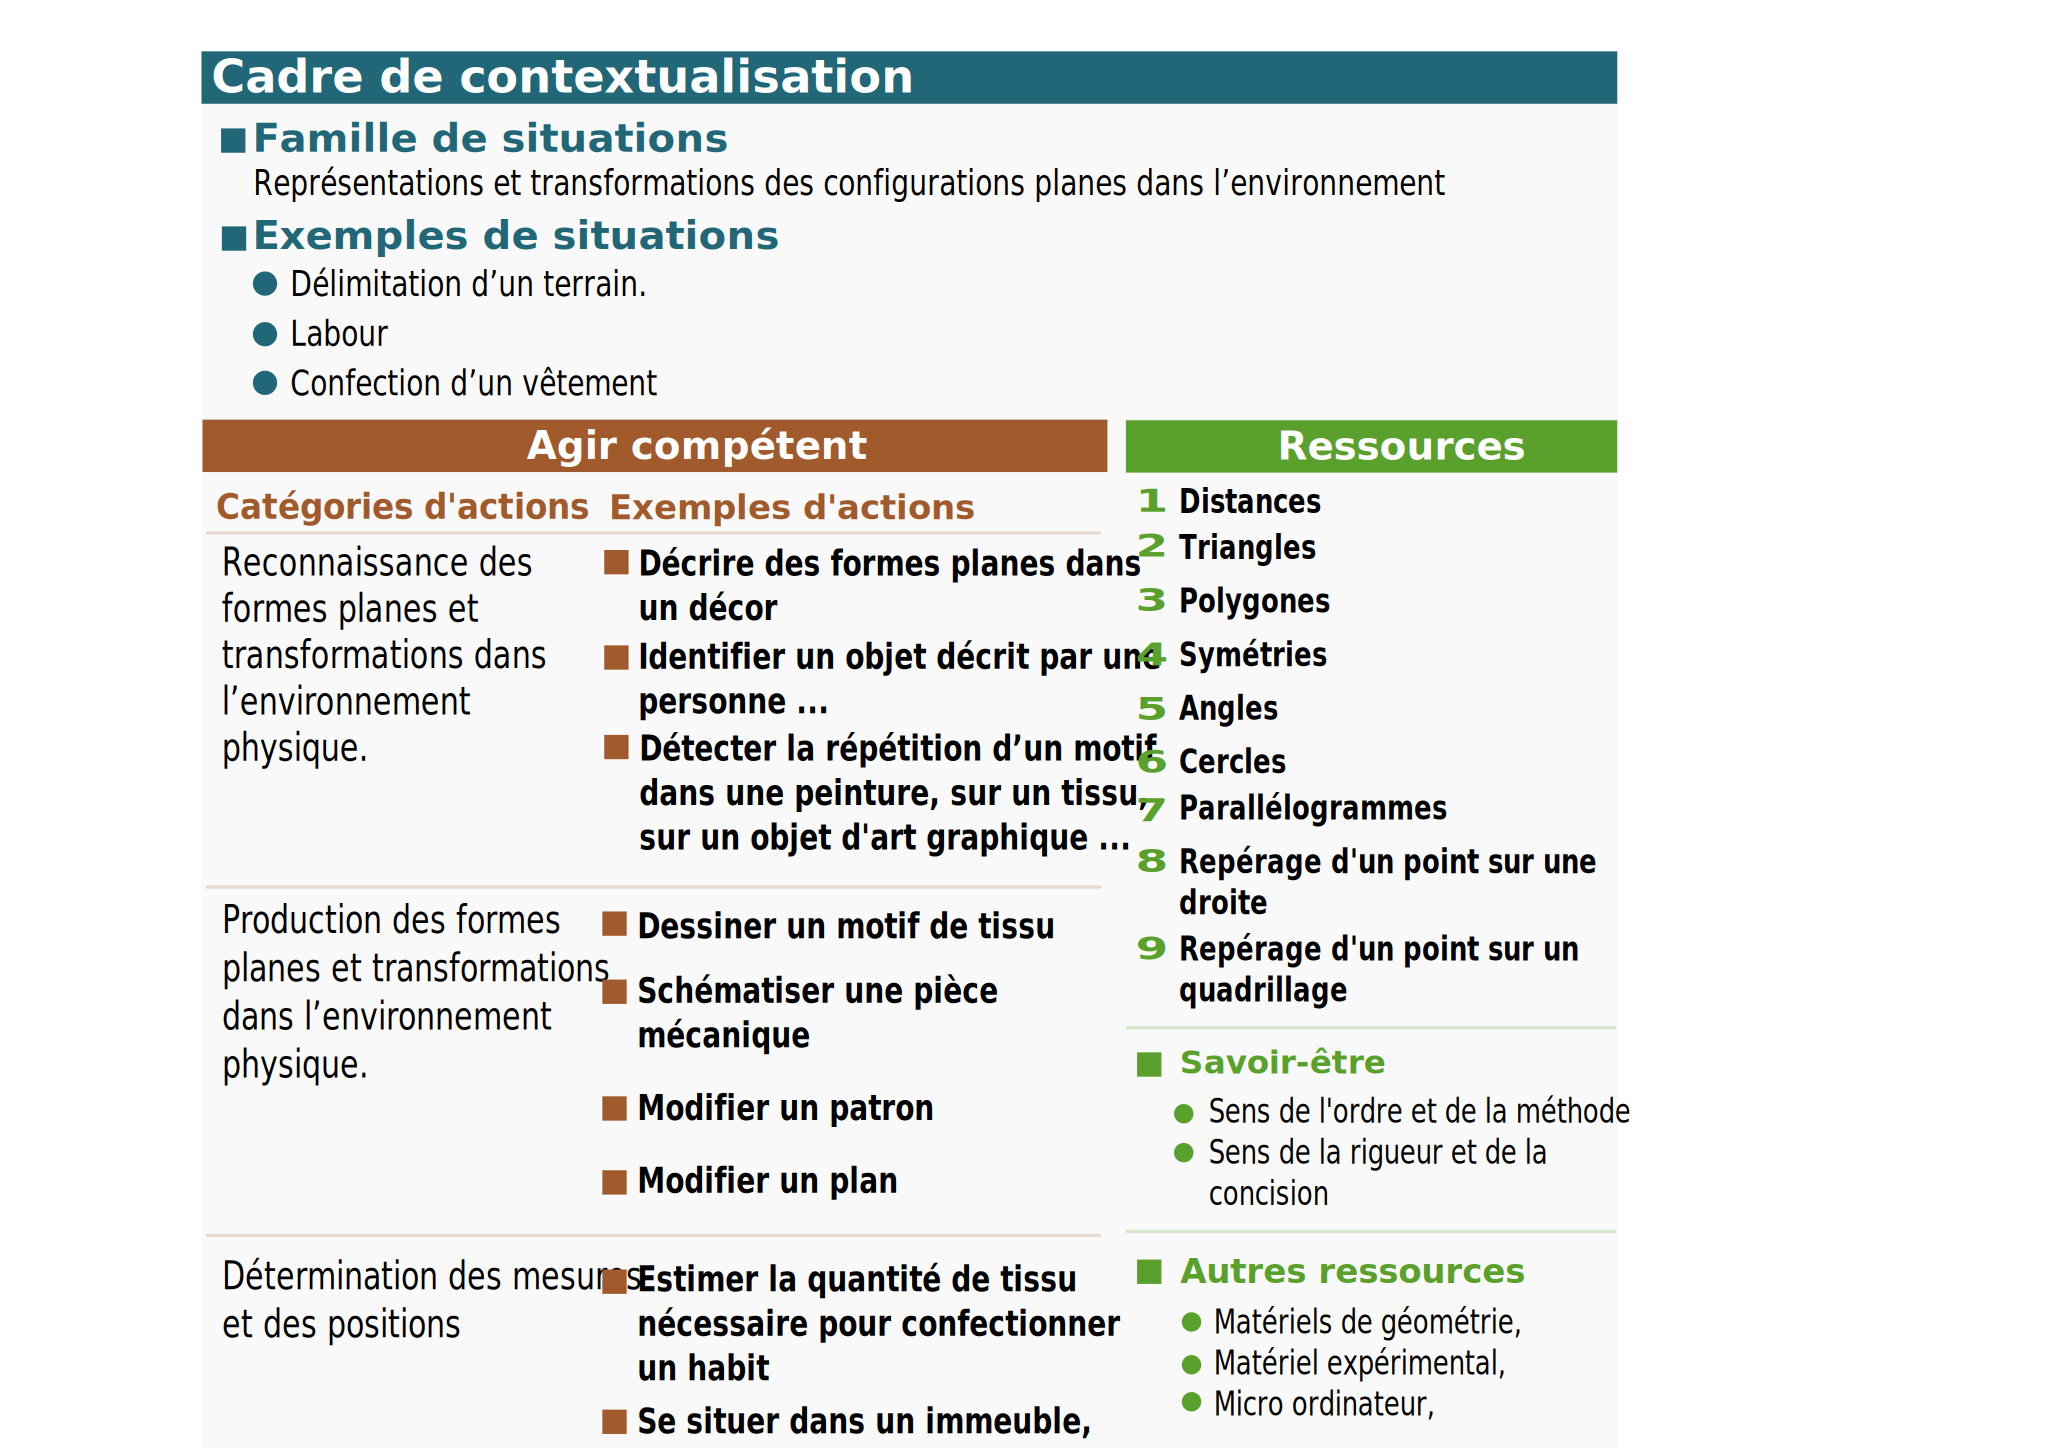
\includegraphics[width=\textwidth]{Module7.pdf} 

\subsection*{}
\addcontentsline{toc}{subsection}{\textbf{Ressource 1}: distances}
\ressource{Dis.pdf}

\savoir
\begin{itemize}
\item Distances de deux points.
\item Inégalité triangulaire.
\item  Caractérisation d'un segment par les distances (Si $M\in\ife{AB}$ alors  MA + MB = AB et si $MA+MB=AB$
alors $M\in\ife{AB}$ ).
\item Caractérisation de la médiatrice d'un segment par l'égalité des distances.
\end{itemize}
\savoirfaire
\begin{itemize}
\item Construire la médiatrice d'un segment à la règle et au compas.
\item Utiliser l'inégalité triangulaire et la caractérisation de la médiatrice pour justifier des inégalités ou des égalités des distances.
\end{itemize}

\subsection*{}
\addcontentsline{toc}{subsection}{\textbf{Ressource 2}: triangles}
\ressource{Tri5.pdf}

\savoir
\begin{itemize}
\item \textit{ Droites particulières dans un triangle} : hauteur, médiatrice, médiane, bissectrice.
\item Somme des angles d'un triangle.
\item \textit{Caractérisation des triangles particuliers}: triangle rectangle, triangle isocèle, triangle équilatéral.
\end{itemize}
\savoirfaire
\begin{itemize}
\item Construction des triangles particuliers.
\item Construction des droites particulières d'un triangle (hauteurs, médiatrices, médianes, bissectrices).
\end{itemize}

\subsection*{}
\addcontentsline{toc}{subsection}{\textbf{Ressource 3}: polygones}
\ressource{Pol.pdf}

\savoir
\begin{itemize}
\item \textit{Polygones usuels} : triangle, trapèze, pentagone, hexagone régulier, octogone régulier, parallélogrammes.
\end{itemize}
\savoirfaire
\begin{itemize}
\item \textit{Caractérisation des polygones particuliers en liaison avec les symétries} : trapèze isocèle, hexagone
régulier, octogone régulier.
\item \textit{Reconnaître et construire un polygone particulier} : parallélogramme, trapèze, losange, hexagone régulier, octogone régulier, pentagone.
\end{itemize}

\subsection*{}
\addcontentsline{toc}{subsection}{\textbf{Ressource 4}: symétries}
\ressource{Sym.pdf}

\savoir
\begin{itemize}
\item Symétries par rapport à un point, symétrie orthogonale.
\item \textit{Propriétés de conservation} : distances, angles, formes, parallélisme, orthogonalité, alignement des points.
\end{itemize}
\savoirfaire
\begin{itemize}
\item Construction des figures symétriques par rapport à une droite ou un point (point, droite, segment, triangle, cercle) ;
\item Utilisation des propriétés de conservation pour justifier une égalité de distance ou angulaire ou l'alignement de 3 points, l'orthogonalité ou le parallélisme de 2 droites ;
\item Remplir un tableau de correspondance dans l'étude des figures symétriques ;
\item Reconnaître une configuration admettant un axe(ou un centre) de symétrie et préciser cet axe (ou ce centre) de symétrie.
\end{itemize}

\subsection*{}
\addcontentsline{toc}{subsection}{\textbf{Ressource 5}: angles}
\ressource{Ang5.pdf}

\savoir
\begin{itemize}
\item Angles complémentaires, angles supplémentaires ;
\item Angles opposés par le sommet ;
\item Angles formés par deux droites parallèles et une sécante ;
\item Angles alternes - internes, angles alternes-externes, angles correspondants.
\end{itemize}
\savoirfaire
\begin{itemize}
\item Utiliser les différentes propriétés pour justifier une égalité angulaire.
\end{itemize}

\subsection*{}
\addcontentsline{toc}{subsection}{\textbf{Ressource 6}: cercle}
\ressource{Cer5.pdf}

\savoir
\begin{itemize}
\item Cercle circonscrit à un triangle, à un rectangle ;
\item \textit{Régionnement du plan par un cercle}: intérieur, extérieur d'un cercle
\end{itemize}
\savoirfaire
\begin{itemize}
\item Position d'un point par rapport à un cercle ;
\item Construction du cercle circonscrit à un triangle, à un rectangle.
\end{itemize}

\subsection*{}
\addcontentsline{toc}{subsection}{\textbf{Ressource 7}: repérage d'un point sur une droite}
\ressource{Repd.pdf}

\savoir
\begin{itemize}
\item Notion d'abscisse relativement d'un point.
\end{itemize}
\savoirfaire
\begin{itemize}
\item Justifier des inégalités de nombre par leur rangement sur une droite.
\end{itemize}

\subsection*{}
\addcontentsline{toc}{subsection}{\textbf{Ressource 8}: repérage d'un point sur un quadrillage}
\ressource{Repq.pdf}

\savoir
\begin{itemize}
\item Vocabulaire ;
\item Notion de couple de coordonnées (entiers relatifs).
\end{itemize}
\savoirfaire
\begin{itemize}
\item Placer sur un quadrillage, un point dont on connaît le couple de coordonnées (entiers relatifs) ;
\item Lire le couple de coordonnées d'un point dans un quadrillage.
\end{itemize}  

